\fakesection{Classification}{\hfill\small\texttt{/src/session\_1/.m}}

\fakesubsection{Two Gaussians}{}

For a binary classifier where the distributions are (assumed or known to be) Gaussian with equal covariance matrices the decision boundary that maximises the posterior probability $P(C_i|x)$ becomes linear. This is independent of the amount of overlap. Trying to get a better boundary would lead to overfitting. In this particular example where $\Sigma_{xx}=\mathbb{I}$ one ends up with a perpendicular bisector of the segment connecting the two cluster means 
$(-1,-1)$ and $(1,1)$, which gives $f(x)=-x$ as a decision boundary.

\begin{figure}[h]
\centering
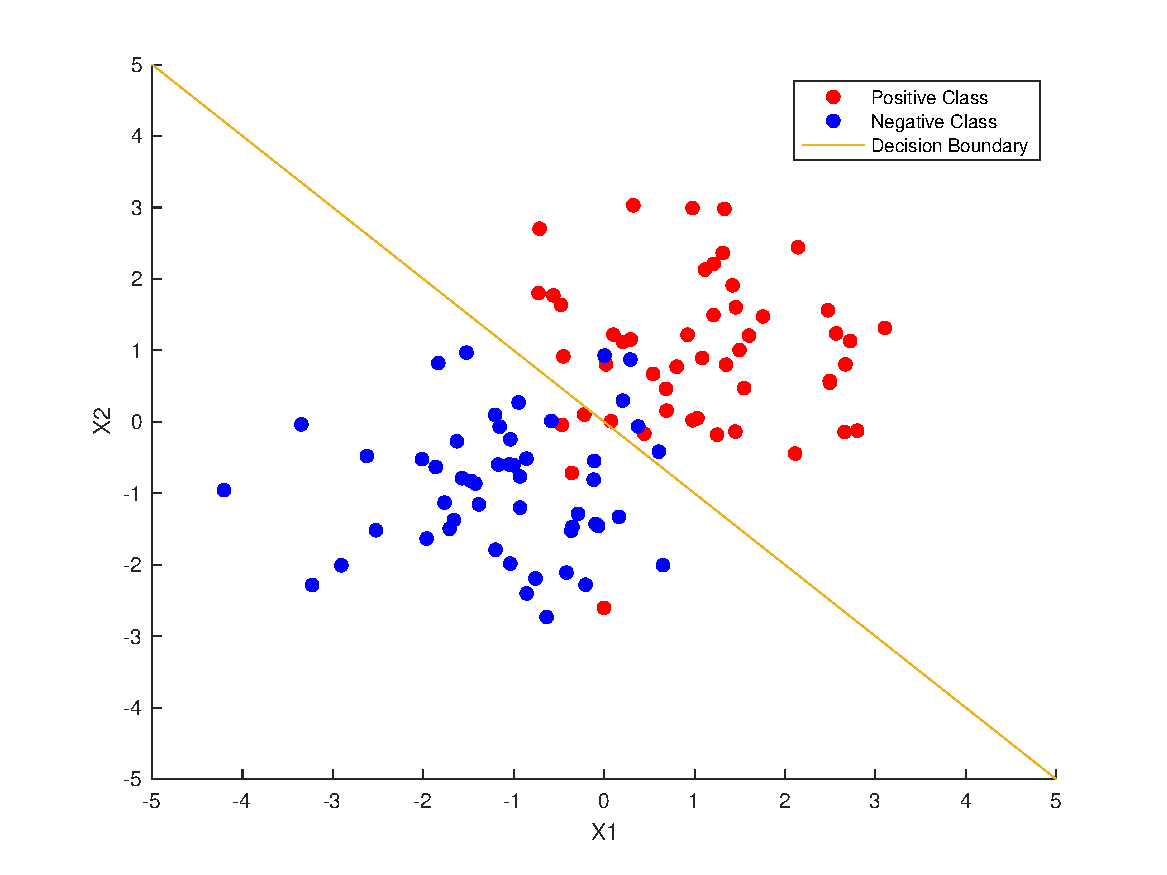
\includegraphics[width=0.6\textwidth]{../src/figures/twogaussians.pdf}
\label{twogaussians}
\caption{Decision boundary for two Gaussian distributions with equal covariance matrices.}
\end{figure}

\fakesubsection{Support Vector Machine Classifier}{}

To deal with the non-separable classification problem in the example one solves the following minimisation problem, where the hyperparameter $C$ controls the tradeoff between maximising the margin and making sure that the data lies on the correct side of that margin :
$$\min_x\quad\frac{1}{2}\cdot w^T\cdot w+C\cdot \sum_{k=1}^N\xi_k$$
\noindent It can readily be seen that for a decreasing $C$ the margin does become larger and that less \textit{`slacking'} is allowed.